\documentclass[a4paper]{article}
\usepackage[affil-it]{authblk}    
\usepackage{graphicx}
\usepackage{tabularx}
\usepackage{epstopdf}
\usepackage{amsmath}
\usepackage{amssymb}
\usepackage{amsfonts}
\usepackage{amsthm}
%\usepackage{endfloat}
\usepackage{float}
\usepackage[sort,compress]{natbib}
%\bibpunct{[}{]}{,}{n}{,}{,}  % https://xianblog.wordpress.com/tag/natbib/ (allows natbib with PNAS)
\usepackage{endnotes}
\usepackage{setspace}
\usepackage{verbatim}
\usepackage[left=2.5cm, right=2.5cm, bottom=2cm, top=2cm]{geometry}
\usepackage{times}
\usepackage{helvet}
\usepackage{courier}
%\usepackage{mathtime}
\usepackage{bm}
\usepackage{url}
%\usepackage{babel}
\usepackage{dcolumn}
\usepackage{multirow}
\usepackage{makecell}
\usepackage{boldline}
\setcellgapes{3pt}
\usepackage[flushleft]{threeparttable}
\usepackage{wrapfig}
\newcommand{\citetapos}[1]{\citeauthor{#1}'s \citeyearpar{#1}}
%%%%%

\usepackage[
  breaklinks=true,
  colorlinks=true,
  linkcolor=blue,anchorcolor=blue,
  citecolor=blue,filecolor=blue,
  menucolor=blue,pagecolor=blue,
  urlcolor=blue]{hyperref}

\usepackage{lineno}
\usepackage{float}
\usepackage[anythingbreaks]{breakurl}



%\begin{document}
%\hspace*{\fill}

%\title{A Large-Area, Spatially Continuous Quantification of Error in Land Cover Maps and Associated Socioeconomic and Environmental Analyses Relevant to Global Change}
\title{A Large-Area, Spatially Continuous Assessment of Land Cover Map Error and Its Impact on Downstream Analyses}
%\title{How Land Cover Errors Can Impact Understanding of Socioeconomic and Environment Phenomena}
\author[1,2,3]{Lyndon Estes}
\author[4]{Peng Chen}
\author[2]{Stephanie Debats}
\author[4]{Tom Evans}
\author[5]{Stefanus Ferreira}
\author[6,7]{Tobias Kuemmerle}
\author[2]{Gabrielle Ragazzo}
\author[2,8]{Justin Sheffield}
\author[9]{Adam Wolf}
\author[2]{Eric Wood}
\author[2,10]{Kelly Caylor}

\affil[1]{Woodrow Wilson School, Princeton University, Princeton, NJ USA}
\affil[2]{Civil and Environmental Engineering, Princeton University, Princeton, NJ USA}
\affil[3]{Graduate School of Geography, Clark University, Worcester, MA USA}
\affil[4]{Indiana University, Bloomington, IN USA}
\affil[5]{GeoTerraImage, Pretoria, RSA}
\affil[6]{Geography Department, Humboldt University, 10099 Berlin, Germany}
\affil[7]{Integrative Research Institute for Transformations in Human-Environment Systems, Humboldt University, 10099 Berlin, Germany}
\affil[8]{Geography and Environment, University of Southampton, Southampton, United Kingdom}
\affil[9]{Arable Labs, Princeton, NJ USA}
\affil[10]{Bren School of Environmental Science and Management, University of California Santa Barbara, Santa Barbara, CA USA}

\date{}
%\contributor{Submitted to Proceedings of the National Academy of Sciences
%of the United States of America}

%%%Newly updated.
%%% If significance statement need, then can use the below command otherwise just delete it.
%\significancetext{Remote sensing-derived land cover maps underpin much research into global environmental change, particularly in the most rapidly developing regions. These maps often contain substantial error, yet inadequate validation data makes it impossible to fully quantify map errors and how they affect our understanding of global change processes. Using a unique, high quality reference map of cropland distribution, this study comprehensively assesses land cover map bias and accuracy in a major agricultural region of sub-Saharan Africa, finding that map errors are strongly correlated with the land cover density, and can propagate substantial errors in downstream global change analyses. Users of land cover maps should select later generation products and aggregate to appropriate resolutions to avoid misleading insights and policies related to global change. }

\begin{document}
\maketitle 

%\begin{article}
\begin{abstract}
{Land cover maps increasingly underlie research into socioeconomic and environmental patterns and processes, including global change. It is known that map errors impact our understanding of these phenomena, but quantifying these impacts is difficult because many areas lack adequate reference data. We used a highly accurate, high-resolution map of South African cropland to assess 1) the magnitude of error in several current generation land cover maps, and 2) how these errors propagate in downstream studies. We first quantified pixel-wise errors in the cropland classes of four widely used land cover maps at resolutions ranging from 1 to 100 km, then calculated errors in several representative ``downstream'' (map-based) analyses, including assessments of vegetative carbon stocks, evapotranspiration, crop production, and household food security. We also evaluated maps' spatial accuracy based on how precisely they could be used to locate specific landscape features. We found that cropland maps can have substantial biases and poor accuracy at all resolutions (e.g. at 1 km resolution, up to $\sim$45\% underestimates of cropland (bias) and nearly 50\% mean absolute error (accuracy); at 100 km, up to 15\% underestimates and nearly 20\% MAE). National-scale maps derived from higher resolution imagery were most accurate, followed by multi-map fusion products. Constraining mapped values to match survey statistics proved effective at minimizing bias (provided the statistics are accurate). Errors in downstream analyses could be substantially amplified or muted, depending on the values ascribed to cropland-adjacent covers (e.g. with forest as adjacent cover, carbon map error was 200-500\% greater than in the foundational cropland maps, but $\sim$40\% less for sparse cover types). The average locational error was 6 km (600\%). These findings provide deeper insight into the causes and consequences of land cover map error, including their potential broader regional and policy consequences, and suggest several recommendations for land cover map users.  
%
%
%These maps can have substantial error that impact , which may impact our understanding of environmental change processes and associated policies is thus of great interest, but is difficult to fully quantify because we lack spatially comprehensive reference data, particularly in the World's most rapidly developing regions. We used a high quality, national-scale cropland map to assess bias and accuracy within the cropland classes of current generation land cover datasets and four examples of ``downstream'' (land cover-dependent) analyses, two related to physical processes (estimates of vegetative carbon stocks and evapotranspiration) and two to socio-economic processes (gridded crop production estimates and agent-based simulation of household food security), at resolutions ranging from 1-100 km. We found that cropland maps have substantial errors below 25 km resolution, with substantial biases and inaccuracies, particularly from maps derived from coarse resolution sensors. In some cases these error metrics remain high even when maps are aggregated to 100 km. These errors can be substantially amplified in downstream analyses (e.g. the carbon and crop production analyses), but in cases where the values of different cover types that underpin the analysis are similar (e.g. evapotranspiration estimates) the results can be relatively insensitive. To avoid these errors, and thus minimize the risk of misunderstanding global change processes or misinforming policy, substantial map aggregation of land cover maps from their base resolution is often needed. NEW TEXT HERE.  
}
\end{abstract}

%\keywords{land cover | bias | remote sensing | agriculture | crop yield | harvested area | carbon | agent-based model | landscape}

%\abbreviations{GTI, GeoTerraImage; SSA, sub-Saharan Africa}
\linenumbers

\section*{Introduction}
\vspace{-0.3 cm}
The functioning of the Earth System is fundamentally connected to the characteristics of land cover \citep{lambin_modelling_1997}. Our increasing modification of the Earth's surface \citep{lambin_dynamics_2003} means that socioeconomic and physical processes increasingly interact through land cover. To fully understand these processes, it is essential to have an accurate understanding of the nature and distribution of land cover \citep{verburg_challenges_2011}. This importance is understood by a growing number of social, economic, and natural scientists, who are using land cover data to advance understanding of food security \citep{lark_cropland_2015,wright_recent_2013, licker_mind_2010}, carbon cycling \citep{asner_high-resolution_2010, gaveau_major_2014}, biodiversity loss \citep{newbold_global_2015, luoto_predicting_2004}, demographic shifts \citep{linard_assessing_2010}, and other important facets of Earth System processes. 

The value of the insights resulting from such studies depends upon the veracity of their underlying land cover data \citep{verburg_challenges_2011}, much as a house requires a solid foundation in order to remain standing. Unfortunately, the evidence indicates that this house has shaky foundations \citep[e.g.][]{fritz_highlighting_2011}. The reason for this is that land cover data can only practically be derived from satellite imaging, which has several important constraints that propagate mapping errors. First, in many regions the spatial arrangement of cover types is smaller than the sensor resolution \citep[e.g. smallholders' fields][]{jain_mapping_2013,debats_generalized_2016,ozdogan_resolution_2006}, or the types of interest are spectrally indistinct from neighboring ones \citep{sweeney_mapping_2015,fritz_identifying_2008}, which are factors that increase mapping complexity \citep{yu_meta-discoveries_2014}. Second, the act of defining a cover class can cause error, in that selected classes may have highly diverse spectral properties \citep[e.g. croplands or savannas;][]{fritz_identifying_2008,verburg_challenges_2011,debats_generalized_2016} and can thus be difficult for the classifier to distinguish. Discretizing a continuous cover type (e.g. dividing a forest into different canopy cover classes) can promote classification error, particularly near class boundaries \citep{foody_status_2002}, as well as confusion about the actual extent of the cover type \citep{sexton_conservation_2015}. Furthermore, class definitions often vary between maps, complicating inter-comparison \citep{kuemmerle_challenges_2013,fritz_identifying_2008}. Third, land cover maps are often used to detect changes \citep[e.g.][]{gross_monitoring_2013}, but seasonal variability and land cover changes can be easily confused. Given these multiple sources of error, land cover maps are often inaccurate at finer scales and disagree widely between products, particularly in the world's most rapidly developing regions \citep{estes_projected_2013,fritz_comparison_2010,fritz_cropland_2011,fritz_need_2013}. These errors limit our ability to obtain granular, mechanistic understanding of processes related to global change. 

These problems with land cover products are known \citep{fritz_comparison_2010, fritz_cropland_2011, see_improved_2015, fritz_mapping_2015,verburg_challenges_2011}, and there are a variety of map improvement efforts underway \citep[e.g.][]{fritz_geo-wiki:_2012, estes_platform_2016}. Likewise, the importance of assessing the accuracy of land cover maps is increasingly recognized, and there are well-developed, best-practice guidelines for gathering and using ground-truth samples to robustly quantify map error \citep{foody_status_2002,olofsson_making_2013,olofsson_good_2014,stehman_global_2012}. Because comprehensive, spatially representative ground truth data are typically unavailable for rapidly changing regions \citep{see_improved_2015,kuemmerle_challenges_2013}, what remains an open question is exactly how much the maps researchers typically use deviate from actual land cover, how this affects our analyses based on these maps, and how this in turn impacts our understanding of environmental change processes.  Our current understanding of map accuracy over such areas is often based on scarce information or top-down "sanity checks" made in comparison to aggregated survey data \citep{yu_meta-discoveries_2014,larsen_taken_2015}.  

Since it is difficult to fully quantify land cover map errors, it is even more challenging to gauge their impact on downstream analyses, where there is substantial risk of error amplification \citep{kuemmerle_challenges_2013}. Although previous studies have examined how map errors propagate, these are primarily assessed using either simulated errors, relative differences in existing land cover maps, or ground validation data covering relatively small areas \citep[e.g.][]{ge_impacts_2007, linard_assessing_2010, quaife_impact_2008, tuanmu_global_2014, schmit_limitations_2006}. 

Fortunately, the recent, explosive growth in public and private initiatives to develop new Earth observing capabilities, which range from small drones\footnote{e.g. 3DRobotics, DJIA} to new high resolution satellite arrays \citep{drusch_sentinel-2:_2012,hand_startup_2015} and better mapping methods \citep{fritz_geo-wiki:_2012,estes_projected_2013,debats_generalized_2016}, are finally providing the means to more comprehensively interrogate the accuracy and biases in the land cover products that have become commonplace in global change research--and which are often used to make policy decisions \citep{searchinger_high_2015}.  

In this study, we take advantage of this recent growth in data to address the call to more thoroughly assess errors in land cover maps \citep{kuemmerle_challenges_2013, olofsson_good_2014,olofsson_global_2012}, and further examine how these errors might impact our understanding of socioeconomic and environmental conditions. Using a unique, high-resolution, high-quality map of South African croplands, which was created by expert mappers delineating individual fields visible within high resolution imagery, we conduct spatially comprehensive, bottom-up analyses to answer the following two questions: 1) What is the extent of error in several widely used land cover products?; 2) How do these errors propagate through downstream biophysical and socioeconomic analyses? 

The answers to these questions provide important insights into how cropland datasets can influence our understanding socioeconomic and environmental processes in South Africa, as well as more broadly throughout sub-Saharan Africa (SSA), where our current knowledge of the extent and distribution of cropland relies heavily on land cover maps \citep[][]{fritz_comparison_2010, see_improved_2015}. 

\vspace{-0.5 cm}
\section*{Materials and Methods}
\vspace{-0.3 cm}
\subsection*{Datasets}
\vspace{-0.2 cm}
In the late 2000s, the South African government commissioned a cropland map that was made by manually interpreting and digitizing fields visible within high resolution satellite imagery \citep{fourie_better_2009}. The resulting vectorized field boundaries provide unique, highly accurate data on field sizes and distribution for 2009-2011. The accuracy of this dataset was evaluated in a previous study \citep{estes_platform_2016}, in which visual assessment of cropland presence/absence was made within 15,225 individual 4 ha plots (25 sub-plots within 609 1 km$^2$ grids) placed over high resolution satellite imagery, and compared to coverage by the vector boundaries. Measured in terms of its ability to distinguish crop fields from other cover types, the results showed these data to be 97\% percent accurate, with user's accuracies of 94\% and 98\% for the cropland and non-cropland classes, and producer's accuracies of 84 and 99\% \citep[see SI for more description, and][]{estes_platform_2016}. 

We used these vector data as a reference for evaluating four land cover products representative of the type commonly used in global change studies and related areas of research. The first was South Africa's own 30 m resolution 2009 National land cover map \citep[SA-LC][]{sanbi_national_2009}, which is typical of the higher-resolution, Landsat-based maps that are created for individual countries \citep[e.g.][]{fry_completion_2009}. Although global-scale, Landsat-derived maps have recently become available \citep{chen_global_2015}, their reported accuracy for cultivated areas is lower (80-85\% user's accuracy) than that achieved by more intensive, national to sub-national products \citep[e.g. 90\% user's accuracy][]{sweeney_mapping_2015}. The second and third were respectively the 300 m GlobCover 2009 \citep{arino_global_2012} and 500 m resolution MODIS land cover \citep{friedl_modis_2010} data (for 2011, the final year of the reference interval), which are widely used global-scale products \citep[e.g.][]{gross_monitoring_2013, shackelford_conservation_2015}. The fourth dataset was the 1 km GeoWiki cropland map for Africa \citep{fritz_mapping_2015}, which fuses the cropland classes of multiple landcover products (including the three assessed here), with the resulting cropland percentages adjusted until their totals sum to match cropland areas reported in national agricultural statistics (this method also incorporated additional categorical training data collected via crowdsourcing). This ``hybrid-fusion'' approach represents the state of the art in mapping agricultural land cover. Since GeoWiki provides a continuous bounded value of land cover (cropland percentage), which cannot be feasibly converted to a categorical value, we converted all other datasets, including the reference vectors, into comparable 1 km gridded percent cropland estimates. 

%is a ``fusion'' product, in that it merges the results of the first three datasets (and several others), using i) the extent of the agreement between each landcover product and ii) each product's reliability, as determined by crowdsourced validation data, to assign a likelihood of cropland presence, and then calibrating that likelihood into a cropland percentage through calibration against national agricultural statistics.  and represents the current state-of-the-art in land cover mapping.  

To develop percent coverage from the cropland reference map, we intersected the original field boundary vector maps with a 1 km grid, and calculated the percent of each cell occupied by fields. In the resulting grid, we masked out areas classified as communal farmland (18.7\% of mapped croplands in the reference data), because only their outer perimeters were digitized \citep{fourie_better_2009}, which risked overestimating cropland extent because the vectors also enclose uncropped areas between adjacent smallholder fields. We also excluded from the analysis areas covered by permanent tree crops, sugarcane plantations, and commercially afforested areas, because these three classes were not common to all five cropland datasets. To remove permanent tree crops (3.1\% of cropland area), we masked out reference vectors labelled as such, and to exclude the other two cover types, which are not included in the reference data, we relied on information from two other datasets. We used a 20 m resolution landcover map of KwaZulu-Natal to mask out the primarily coastal sugarcane farms \citep[93-100\% user's and 76-98\% producer's accuracy for sugarcane classes;][]{geoterraimage_2011_2013}, and used the SA-LC dataset to filter out areas of commercial afforestation, which are mainly located in South Africa's montane areas and do not overlap with arable croplands. In both cases, we aggregated these classes, and then masked out any 1 km pixels that had $>$0\% cover of each class. The resulting masked reference grid covered 90\% of South Africa (1,081,000 km$^2$), of which 104,304 km$^2$ was cropland. 

We extracted the cropland classes from SA-LC, MODIS, and GlobCover, and converted these into percent cropland estimates at 1 km resolution. Both MODIS and GlobCover had mixed/mosaic classes of cropland and other covers, thus we followed \citet{fritz_mapping_2015} by creating upper, mean, and lower cropland estimates from these classes to produce three versions of the gridded percentages. We used the mean map for the main analysis, but estimated error variability using all three versions (SI).

\vspace{-0.3 cm}
\subsection*{Assessment of cropland map errors}
\vspace{-0.2 cm}
We first evaluated the quality of the land cover product-derived percent cropland maps (hereafter referred to as the ``test maps''). Instead of the standard confusion matrix-based accuracy metrics \citep{olofsson_good_2014,olofsson_making_2013}, which apply to categorical land cover maps, we assessed the bias and accuracy of the test maps based on the gridded residuals that resulted when each test map was subtracted from the reference map. Here bias is the mean residual value, weighted by the density of reference cropland, and accuracy is the mean of the absolute values of residuals (also weighted by cropland density), thus lower values signify higher accuracy. We calculated these metrics for the original 1 km resolution, and for maps that were further aggregated to 5, 10, 25, 50, and 100 km resolutions, in order to evaluate how bias and accuracy changes with observational grain. For these aggregated maps, we applied a further weight in calculating error metrics, the number of pixels contributing to each aggregated pixel, to prevent pixels close to national boundaries or where non-target cover types were masked out from having outsize influence on the statistics. 

We also assessed how land cover pattern impacts map performance by modeling the correlation between map accuracy and cropland density.  To evaluate this relationship, we used magisterial district boundaries (n=354, mean area=3,445 km$^2$; SI) to provide a landscape-scaled unit for calculating characteristic cover density. We filtered out pixels with $<$0.05\% (0.5 ha) cropland, to prevent the much larger areas of non-agricultural districts from dominating the signal, extracted the absolute values of test map errors and corresponding reference cropland percentages, and calculated their district-wide means. The relationship between mean absolute error (response) and cropland density (predictor) was then modeled using a generalized additive model \citep{hastie_generalized_1990}, with each district weighted by its number of agricultural pixels \citep{wood_mgcv:_2001}. To account for potential spatial autocorrelation, we fit a two-dimensional smoothing spline to the coordinates of each district's centroid.

\vspace{-0.3 cm}
\subsection*{Impact of map error on downstream analyses}
\vspace{-0.2 cm}
We then used the reference and test maps to conduct four analyses typical of global change research: 1) estimation of carbon stocks, 2) simulation of evapotranspiration, 3) disaggregation of crop yield and production, and 4) simulating household dynamics using an agent-based model. The first and third analyses were relatively simple, in that the variable(s) of interest were mapped onto land cover using empirical relationships. The second and fourth relied on more complex numerical methods, where land cover was one of several variables needed to run each model. For the simpler analyses, we examined how results were influenced by map aggregation, while for the more complex cases, our assessments were confined to each numerical model's standard output resolution. 

\vspace{-0.3 cm}
\subsubsection*{Estimating vegetative carbon stocks}
\vspace{-0.2 cm}
To understand the carbon cycle and climate forcing due to land cover change, it is important to have accurate, high resolution maps of vegetative carbon stocks \citep[][]{searchinger_high_2015}. One widely used vegetative carbon dataset is that of \citep{ruesch_new_2008}, who mapped estimated carbon density values for different vegetation types to the classes of a global land cover product. The resulting data were intended to provide a baseline for climate policy by the Intergovernmental Panel on Climate Change (IPCC), as well as input to other land use and biogeochemical analyses \citep{ruesch_new_2008}. 

%\vspace{-1 cm}
We followed this method to create vegetative carbon maps for South Africa. Since our cropland percentage map provided no information on surrounding cover, we developed several variants representing potential surrounding cover types by assigning the average carbon densities of five biomes (forest, secondary forest, shrubland, grassland, and sparse vegetation \citep{ruesch_new_2008}) to the non-cropland fraction of our maps. These hypothetical maps represented the range in potential carbon densities, and allowed us to investigate how carbon estimates can vary as a function of i) test map errors and ii) the properties of neighboring cover types. We multiplied cropland densities by cropland fractions and added these to each of the five other densities multiplied by the residual non-cropland fractions to create five different carbon density maps. We aggregated each carbon map up to 5, 10, 25, 50, and 100 km resolutions for scaling comparisons (SI). 

To assess carbon estimation error, we subtracted test map-derived carbon maps from those based on the reference map, and calculated bias and accuracy scores using the method described for the cropland maps (see previous section). 

\vspace{-0.3 cm}
\subsubsection*{Estimating evapotranspiration}
\vspace{-0.2 cm}
Accurate estimation of hydrological fluxes is critical to understanding how land-atmosphere interactions impact the climate system and runoff \citep{liang_simple_1994}. Land surface hydrological models are used to simulate these processes, and depend on land cover maps to provide information on the characteristics of vegetation and other materials covering the surface, as these govern the rates of runoff, infiltration, and evapotranspiration. We used the Variable Infiltration Capacity \citep[VIC;][]{liang_simple_1994} land surface hydrology model run with the Africa Flood and Drought Monitor's meteorological data \citep{sheffield_drought_2013} to produce monthly gridded evapotranspiration estimates for South Africa for the years 1979-2010 at 25 km resolution. VIC's land cover scheme (derived from AVHRR) provides values for leaf area index (LAI), plant rooting depth, aerodynamic roughness, and several other variables that the modeluses to partition water vapor fluxes into their evaporative and transpirative components. We adjusted VIC's base map so that its cropland fractions matched those of the 25 km reference and test maps (each reprojected and resampled to VIC's 0.25$^{\circ}$ resolution), then ran one instance of VIC for each of the five land cover schemes. We then compared the mean annual ET produced by the reference map variant with those from the test maps to assess the degree to which map errors impact evapotranspiration values. 

\vspace{-0.3 cm}
\subsubsection*{Disaggregating crop yield and production statistics}
\vspace{-0.2 cm}
The spatial variability of crop yield and production is critical for understanding food security, trade, and the potential for agricultural expansion and intensification \citep{licker_mind_2010,monfreda_farming_2008}. The most reliable source of such data are national to sub-national agricultural statistics, often available only at relatively coarse-scaled administrative boundaries. To obtain higher spatial resolutions, disaggregation of these statistics using gridded land cover data is common \citep{ramankutty_farming_2008, monfreda_farming_2008,schierhorn_post-soviet_2013}. 

We used these methods to first disaggregate the harvested area for maize (South Africa's largest crop \citep{estes_projected_2013}) onto our cropland maps, followed by yields, which were assigned to cells having harvested areas greater than zero. The first step in this process entails adjusting cropland percentages so that their totals match census-derived cropland area estimates \citep{ramankutty_farming_2008,schierhorn_post-soviet_2013}. In place of census statistics, we used the reference map to calculate total cropland areas for South Africa's nine provinces, then adjusted the pixel-wise cropland percentages in the four test maps so that their province-wise sums matched these totals (SI). We then followed \citetapos{monfreda_farming_2008} procedure for disaggregating maize \citep[South Africa's largest crop;][]{estes_comparing_2013} planted area and yields onto the reference and adjusted test maps. The necessary statistics were obtained from magisterial district-level agricultural censuses conducted for the year 2007 \citep{statistics_south_africa_building_2007}. 

We then used these two layers to calculate maize production, and further aggregated the yield and production grids to 5, 10, 25, 50, and 100 km resolutions before quantifying the bias and accuracy of each test map's yield and production values. In this case, we could not convert cell-wise errors into percentages of the reference map values (because many cells had zero values for one map but not the other), so we calculated bias and accuracy from the map residuals and then normalized their values to the reference map means. 

%\indent To create the gridded maize yield and production maps, we followed Ramankutty et al. \citep{ramankutty_farming_2008} to first calibrate the test cropland maps against cropland areas reported by administrative-level agricultural censuses. 

\vspace{-0.3 cm}
\subsubsection*{Agent-based simulation of household food security }
\vspace{-0.2 cm}
Spatially-explicit agent-based model (ABMs) are frequently employed to understand land use decision-making, to analyze socio-ecological system dynamics, and to test policy impact \citep{berger_creating_2006}. To obtain robust insights, it is important to calibrate an ABM to empirical data describing the characteristics of land and land users, so that the model realistically represents the social and biophysical features of the study region \citep{berger_creating_2006}. 

In our example, we used an ABM of household food security that simulates food production by individual farming households \citep[the agents; ][]{chen_dependency_2013}. The model (described in more detail in the SI) is initialized so that each household is allocated a share of cropland, based on household number and cropland area estimated derived from survey statistics. Annual household crop production (maize) is simulated as a function of its field area, local weather, soil properties, and management actions, all of which can vary between households. The initialization process iteratively assigns households to the landscape as a function of neighbor and cropland proximity, ensuring that households are grouped into communities and that their fields are within a realistic proximity. To achieve this, the model first randomly places 100 households onto the simulated landscape, allocating each household its required cropland pixels, which must be within 1.5 km of the household. This process is iterated until all households are assigned cropland, or all available cropland is allocated. The model is considered to be well-calibrated when all households are allocated cropland, and all cropland is allocated to households. 

Like many spatial ABMs, the model is computationally intensive and requires high spatial resolution to match the scale of individual fields, and therefore applied to smaller regions (e.g. districts). To meet these computational needs, we selected four contiguous magisterial districts (1,040-1,343 km$^2$) in eastern South Africa with similar climate and 28-45\% of cropland coverage. To create cropland surfaces for each district, we disaggregated all five cropland maps into 100 m binary cropland/non-cropland cover maps, and then ran the model separately for each district and with each cropland map (20 simulations total). To examine how map errors impacted the land allocation process and household food production estimates, we calculated three variables: the percent of unallocated cropland, land deficit, and food deficit, which respectively represent: 1) the share of district total cropland that was not assigned to any household (a measure of the model's effectiveness in matching households to available cropland); 2) the total area of cropland that should have been allocated to households in each district but wasn't (due to mismatches between the cropland map and the survey-based estimates of total cropland holdings); 3) the percentage shortfall in the average amount of food production that should have been produced by each household but wasn't because of the land deficit. 

\vspace{-0.3 cm}
\subsection*{The impact of map error on identifying specific locations}
\vspace{-0.2 cm}
The bias and accuracy metrics reflect the degree to quantitative estimates are influenced by land cover map errors. However, land cover data may also be used to identify specific locations \citep[e.g. areas of high agricultural potential and low ecological cost;][]{estes_reconciling_2016}, as opposed to general quantities. It is therefore important to also assess how map errors can impact the spatial accuracy of maps, or the ability to accurately locate specific features of interest. To evaluate this, we calculated the mean Euclidean distance (in km) between pixels representing a specific feature within the test maps relative to their nearest neighboring pixels representing the same feature in the reference map. The features in this analysis were simply those locations falling within the upper deciles of a) cropland cover, b) carbon density (based on the average carbon density of non-crop vegetation types), and c) crop yield. We confined this analysis to the 1 km resolution maps, as higher spatial resolutions are typically required when maps are used to identify locations rather than estimating quantities \citep[e.g.][]{estes_reconciling_2016}.  

\vspace{-0.5 cm}
\section*{Results}
\vspace{-0.3 cm}
\subsection*{Cropland map errors}
\vspace{-0.2 cm}
Our 1 km reference cropland map indicated that crop fields covered 104,304 km$^2$ (nearly 10\%) of the total study area in the 2009-2011 time period, with corresponding cropland area estimates of 131,390, 82,358, 77,090, and 110,272 (GeoWiki) km$^2$ resulting from the SA-LC, GlobCover, MODIS, and GeoWiki maps, respectively. Cropland area estimates from both the reference and test maps were constant for all levels of aggregation. 

Subtracting each test map from the reference maps created pixel-wise residuals, where negative and positive values respectively represent overestimates and underestimates by the test map (Fig. 1A). The most pronounced errors were in the MODIS and GlobCover maps, which showed large positive residuals in the center of the country where cropland is most concentrated (blue areas in Fig. 1A), and negative residuals (red areas) along the eastern and northern margins.
These patterns translated into substantial map bias (Fig. 1B), with GlobCover and MODIS mean error exceeding 45\% and 25\% respectively at 1 km resolution, meaning that each map tends to underestimate cropland by that amount at that resolution. This bias declined with each level of map aggregation, being reduced to nearly 15\% for GlobCover and 5\% for MODIS at 100 km. The magnitude of mean absolute error (MAE) was somewhat higher in all cases. The GeoWiki map, in contrast, was the least biased overall, showing just a $\sim$7\% bias at 1 km and near 0 for all other scales of aggregation, although its accuracy (23\% MAE) was only half as good as SA-LC's at 1 km (11\% MAE), which despite its uniform overestimation bias (Fig. 1A) was the most accurate map at aggregation scales $<10$km. Above this, GeoWiki became slightly more accurate, having $<$5\% MAE at 100 km resolution. The reason GeoWiki had relatively poor accuracy at 1 km resolution was due to the high heterogeneous error pattern, which traded between positive and negative residuals over short distances, thereby inflating MAE at this scale.  

\begin{figure*}[!ht]
%\begin{wrapfigure}{c}{1\textwidth}
\centerline{\includegraphics[width=1\textwidth]{figures/figure1.pdf}}
\vspace{-0.15 cm}
\caption{(A) Errors in the percent cropland estimates resulting from each of the four test maps relative to the reference map at different scale of pixel aggregation. Rows indicate the test map being assessed (by subtraction from the reference map), while columns refer to resolution of aggregation. White indicates areas where areas under communal farmlands or permanent tree crops were removed from analysis. (B) The bias (mean error) and accuracy (mean absolute error [MAE]) of each test map at each scale of aggregation, weighted by the percentage cropland in each cell of the reference map. Bias estimates are indicated by the semi-transparent bars, accuracy (lower is more accurate) by the solid bars, with bar colors coded to specific cropland maps.}
\label{afoto1}
\end{figure*}

%\subsection*{Relationship between map error and cropland density}
The generalized additive model revealed primarily non-linear relationships between district MAE and cropland density that were best approximated by a first order polynomial function of cropland density (for all four cropland maps: p$<$0.001 on both terms of quadratic and on smoothing function applied to district centroids; $>$ 85\% deviance explained). Map accuracy was typically lowest at intermediate levels of cropland density (50-60\% cover) for all but the GlobCover map (where accuracy continues to decline with cropland cover), and was highest where the landscape is dominated either by cropland or by another type (Fig. 2). In other words, accuracy was lowest when cropland cover was mixed evenly with other cover types. GlobCover's accuracy continued to decrease with cropland density because the dominant agricultural cover class contributing to the test map was defined as 50-70\% crops mingled with other vegetation, thus the maximum percentage was constrained by this mixture range.  

%\vspace{-0.75 cm}
%\begin{wrapfigure}{r}{0.5\textwidth}
\begin{figure}[!h]
%\centerline{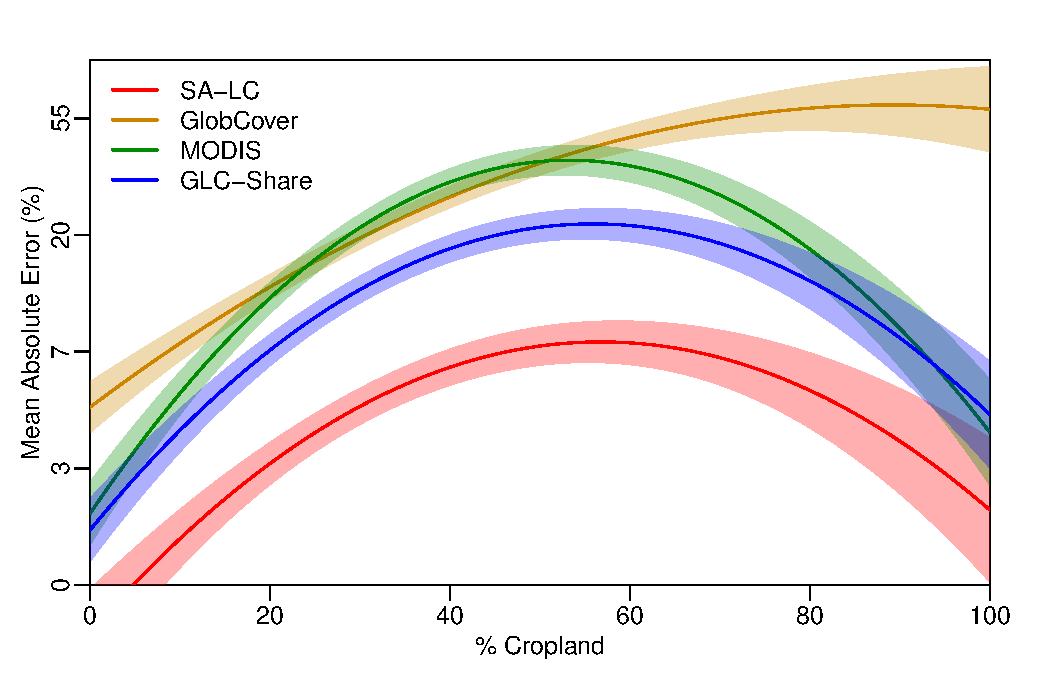
\includegraphics[keepaspectratio,scale = 0.4]{figures/biases_md_lnorm_gam_mu0.pdf}}
\centerline{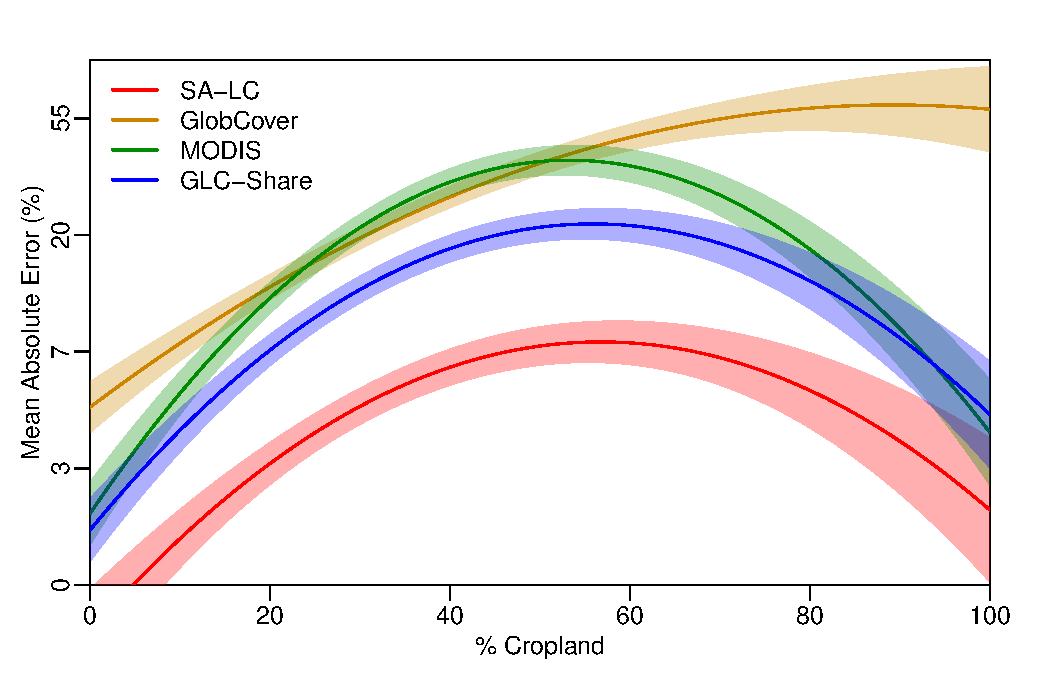
\includegraphics[width=.7\textwidth]{figures/biases_md_lnorm_gam_mu0.pdf}}
\caption{The relationship between map accuracy (the mean absolute error) in test maps and the actual cropland cover within agricultural landscapes (reference map pixels having $>$0.5\% cropland), here defined by the boundaries of magisterial districts (n = 345), as fit with a generalized additive model. Prediction curves are color-coded to the different test maps, with the solid line indicating predicted absolute bias, and the lighter shading the standard error of the coefficients.}\label{afoto2}
\end{figure}
%\end{wrapfigure}
%\vspace{-0.75 cm}


\vspace{-0.3 cm}
\subsection*{The impact of map error on downstream analyses}
\vspace{-0.2 cm}
\subsubsection*{Carbon estimates}
\vspace{-0.2 cm}
The spatial patterns of test map errors transmitted into substantial carbon estimation errors, with the sign varying as a function of the density of carbon adjacent to croplands (SI). Where cropland was underestimated and the surrounding cover type was more carbon dense than cropland, carbon density was overestimated, but when the cover type was less dense than croplands (e.g. sparse vegetation), then carbon density was underestimated. The inverse was true where cropland was overestimated. 

The magnitude of carbon errors varied as a function of the carbon density of surrounding cover, as demonstrated by the bias statistics (Fig. 3). Bias was near zero when grassland was the adjacent cover type (SI), as its carbon density is nearly the same as cropland. However, when forest was adjacent then bias was a three- to five-fold multiple of cropland map bias (Fig. 1B). At the most extreme, GlobCover's bias was -276\% at 1 km, but even SA-LC and GeoWiki had biases of 22\% and -50\%, respectively. Bias could be substantial even for the least carbon dense vegetation type (sparse), as evidenced by the 15-25\% mean error at 1 km for MODIS and GlobCover under this class.  The mean bias across the different potential adjacent vegetation classes ranged between -20 for GeoWiki and -123\% for GlobCover at 1 km (with MODIS in between these), while SA-LC's average bias was 11\%.  Biases declined fairly rapidly with aggregation, with all datasets having an average (across cover types) bias magnitude of $<$10\% at $\geq$25 km of aggregation, except for GlobCover, which was -12\% at 100 km (SI).  As with cropland percentages, GeoWiki produced the least biased carbon density estimates above 1 km resolution. 

%\vspace{-0.75 cm}
\begin{figure}[!h]
%\begin{wrapfigure}{r}{0.5\textwidth}
%\centerline{\includegraphics[keepaspectratio,scale = 0.4]{figures/figure3.pdf}}
\centerline{\includegraphics[width=0.55\textwidth]{figures/figure3.pdf}}
\caption{Biases and accuracies (mean absolute errors) of carbon densities derived from cropland maps, calculated as percents relative to the reference map. Bias estimates (represented by symbols) fall within the semi-transparent floating bars, while accuracies are contained in the solid bars. Bar colors are coded to specific cropland map, symbols indicate which cover type was used to calculate cropland-adjacent carbon density. The bar represents the mean biases calculated across each of the 5 cover types. Shrubland and grassland bias values were near zero, while secondary forest values were close to forest values, and thus these are not shown for display clarity (but see Table S2). MODIS and GlobCover values at 1 km exceeding the plot's Y limits are provided near their truncated tops.}
\label{afoto}
\end{figure}
%\end{wrapfigure}

In terms of accuracy, MAE values were essentially the same as bias magnitudes, except for GeoWiki's, which were twice as large. The average MAE across vegetation classes was 47\% at 1 km, dropping to $<$10 only with 25 km of aggregation. In contrast, SA-LC's carbon estimates were twice as accurate at 1 km, and were slightly more accurate up to 25 km of aggregation were GeoWiki achieved parity.  

\vspace{-0.3 cm}
\subsubsection*{Evapotranspiration estimates}
\vspace{-0.2 cm}
Compared to the carbon analysis, the bias and accuracy in evapotranspiration (ET) calculated using the VIC model was negligible, averaging less than than +/-2\%. However, there were several error hotspots in the resulting ET residual maps (Fig. 4). The most pronounced of these were the 5-15\% overestimates in the center of the country caused when VIC was initialized with MODIS and GlobCover, while overestimates along the southern and western coasts reached 25\%. These locations correspond primarily to the margins of major crop production regions--in the center is the westernmost boundary of the summer rainfall growing region, marked approximately by the 400 mm isohyet, where maize is the primary crop. The west coast hotspot falls at the western edge of the wheat-dominated winter rainfall region \citep{hardy_rainfed_2011}, where growing season rainfall is approximately 200 mm. 

SA-LC and GeoWiki also resulted in ET errors estimates along the southern and western coasts, but here the tendency was to underestimate ET, while biases in the center of the country were either negligible to absent.  All but MODIS underestimated ET by 5-15\% in the northern tip of the country.  

%\vspace{-0.75 cm}
\begin{figure}[h]
\centerline{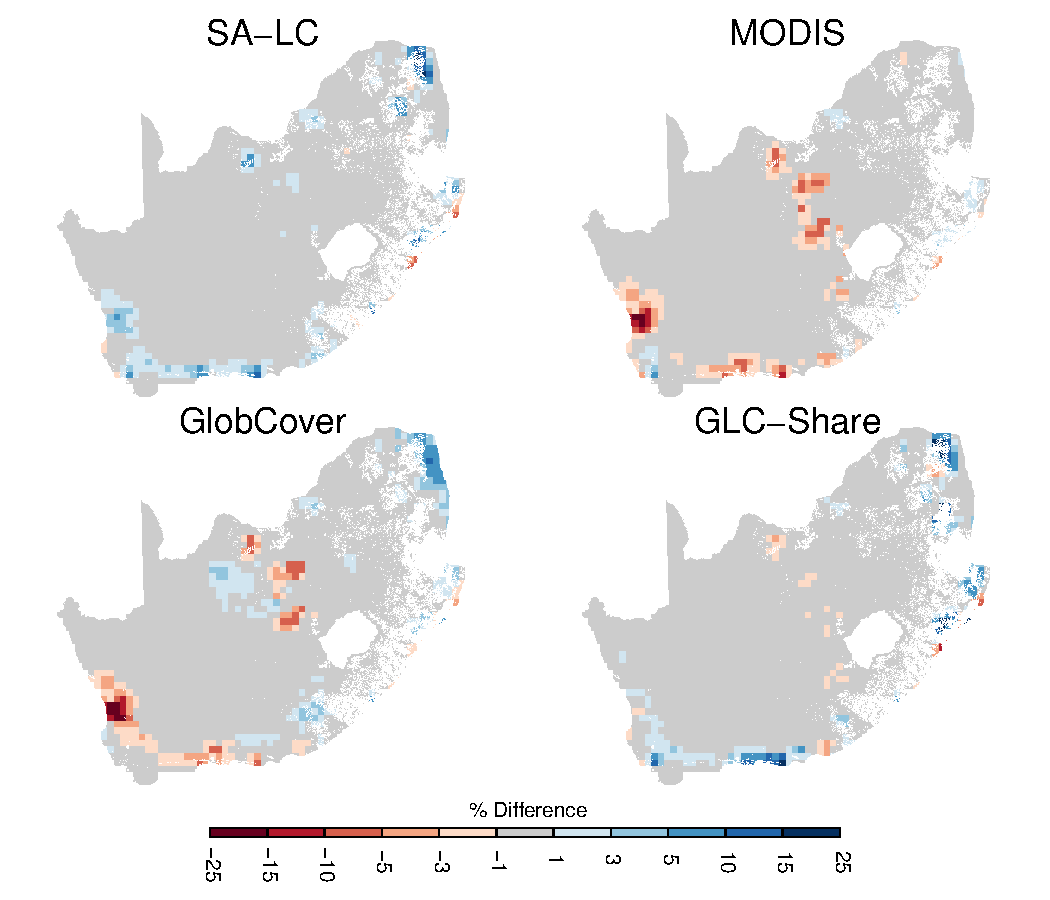
\includegraphics[width=.6\textwidth]{figures/et_bias_map.pdf}}
\caption{Differences in annual mean evapotranspiration estimates from 29-year runs of the VIC land surface hydrology model when initialized with LAI response curves derived from the reference map, versus those from the four test maps.}\label{afoto}
\end{figure}

\vspace{-0.3 cm}
\subsubsection*{Downscaling crop yield and production data}
\vspace{-0.2 cm}
Maize yields disaggregated onto the test maps showed some marked differences relative to the reference map, but only at the margins of the major crop production areas where cropland is sparser (SI). These differences resulted when a yield value was mapped onto a grid cell where the reference map had no harvested area, and thus zero yield. In more densely cropped areas, such discrepancies were less frequent because both the reference and test maps were both likely to have some maize harvested area, and therefore a yield value.  Yield biases were thus fairly low (and accuracy high), with the largest being 20\% for MODIS at 1 km, following by GlobCover with 10\% (Fig. 5). These dropped to $<$10\% with aggregation.  

Production biases were generally higher, but still low, for most datasets, with the exception of GlobCover, which had a large underestimation bias of $>$60\% (relative to mean production) at 1 km, which remained above 10\% even at 100 km of aggregation. MODIS production bias was above 20\% at 1 km, but declined to below 10\% at higher levels of aggregation.  

In contrast, the accuracy of production estimates was poor. Here all datasets but SA-LC had MAE values of $\geq$30\% below 25 km of aggregation (Fig. 5), reaching as high as 100\% for GlobCover at 1 km, followed by 65\% for MODIS and 45\% for GeoWiki. SA-LC estimated production was most accurate, having between 10-20\% MAE between 1 and 10 km, and $<$10\% at 25 km and higher.  This low accuracy relative to the gridded yield measures relates to the disaggregation process for harvested area, which allocates a fractional value to each pixel, which is itself a fraction. The process of adjusting the gridded values so that their totals match reported statistics does relatively little to correct the map's underlying commission or omission errors, and this constraint in fact appears to shorten the distance between negative and positive residuals (SI), thereby increasing absolute errors.  

%\vspace{-0.5 cm}
\begin{figure}[!ht]
%\vspace{-0.75 cm}
\centerline{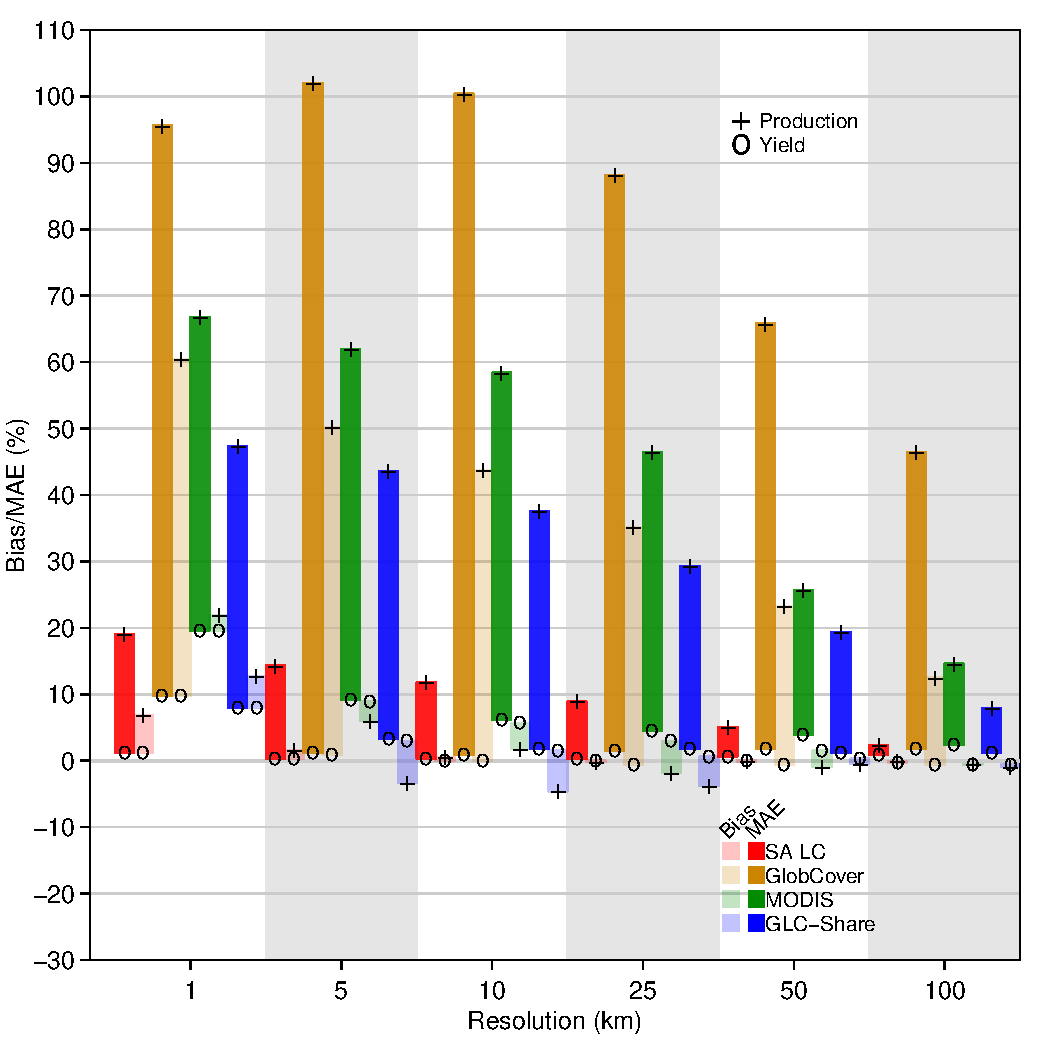
\includegraphics[width=0.55\textwidth]{figures/yield_prod_bias.pdf}}
\caption{Bias (mean error) and accuracy (mean absolute error [MAE]) in disaggregated maize yield and production estimates. Bias estimates (represented by symbols) fall within the semi-transparent bars, mean absolute errors in the solid bars, with bar colors coded to specific cropland maps.  Symbols code the different variables (production and yield), normalized to their respective means.}
\label{afoto}
\end{figure}

\vspace{-0.3 cm}
\subsubsection*{Agent-based model of household food security}
\vspace{-0.2 cm}
In terms of impact to agent-based model simulation, where cropland map errors were negative (indicating a cropland overestimate by the test maps), the percent of land left unallocated had a straight one-to-one relationship with the percentage of overestimation (Fig. 6A). When cropland was underestimated, all croplands were allocated up until the underestimation exceeded 50\%. The MODIS-based simulation for districts 1 and 2 was most pronounced for this tendency, with 5-10\% of cropland remaining unallocated despite the fact that the majority of households were not assigned cropland (because cropland was underestimated by 85\%). This non-linear relationship occurred because croplands tend to cluster, and when underestimated clusters tend to be small and isolated, they are more likely to fall outside of the search radius used by the model for allocating fields to households when they are initially seeded onto the landscape. 

Land deficit (the total area of cropland that should have been allocated to households in each district, but wasn't) increased exponentially in relation to cropland underestimation--reaching around 800\% for MODIS in districts 1 and 2 (Fig. 6B)--and would become infinite in the case of a 100\% underestimate. This contrasted with food deficit (the percentage shortfall in the average amount of food production that should have been produced by each household but wasn't), which increased linearly with the percentage of cropland underestimate (Fig. 6C). 

%randomly siting 100 household agents within each district, and allocating the nearest two cropland pixels to each household. The remaining agents are then iteratively assigned unallocated cropland pixels within a 1.5 km radius of existing agents' fields, and this process continues until all agents are assigned cropland, or all available cropland is allocated. This initialization process 
%\FloatBarrier

\begin{figure}[ht]
\centerline{\includegraphics[width=.55\textwidth]{figures/figure6.pdf}}
\caption{Biases in agent-based model results relative to the district-wise errors (as a percent) in total cropland area, in terms of A) the percent of cropland in each district that was not allocated to any household, B) the land deficit, or the total area of cropland that should have been allocated to households in each district but wasn't (expressed as a percent of total district cropland, as determined by test maps), and C) the food deficit, or the percentage shortfall (relative to the reference simulation) in mean household food production resulting from inadequate cropland allocation. Dot sizes correspond to district numbers, colors represent the land cover map.}
\label{afoto}
\end{figure}

\vspace{-0.3 cm}
\subsection*{Location errors}
\vspace{-0.2 cm}
The average distance between areas containing the highest cropland densities (upper decile) in the reference map and those delineated by the test maps ranged from 1.1 km for SA-LC to 18.2 km for GlobCover, with MODIS (10.1 km) and GeoWiki (2.8 km) having intermediate displacements (Fig. 7). Locational errors in maps indicating the highest yielding areas showed a similar pattern, with a range of 0.8-14.2 km (SA-LC and GlobCover) and intermediate errors of 5.8-7.5 km (GeoWiki and MODIS). For areas of highest carbon density, locations identified by the MODIS-derived map were most distant from those shown by the reference map (11.3 km), followed by GeoWiki (7.4 km), GlobCover (6.8 km), and SA-LC (3.7 km).   

%The analyses above primarily dealt with impact of landcover map errors on estimating quantitative values from maps. However, there are many applications in which land cover data are needed to identify specific locations, such as areas to be targeted for development, where quantitative information is used to target specific locations \citep{estes_reconciling_2016}. 

\begin{figure}[!ht]
\centerline{\includegraphics[width=.55\textwidth]{figures/location_offset.pdf}}
\caption{Average nearest neighbor distances (in km) between pixels representing features identified by the reference map versus those identified from the test maps. Bar colors indicate the different features (and thus contributing maps), which were delineated by selecting pixels with values greater than the 90th percentile: densest cropland (solid bars); highest maize yield (medium transparent bars); highest carbon density (most transparent bars).}   
\label{afoto}
\end{figure}


\vspace{-0.5 cm}
\section*{Discussion}
\vspace{-0.2 cm}
%What We Did and how it is different

The preceding analyses contributes to existing work investigating land cover map error and its consequences \citep[e.g.][]{fritz_highlighting_2011,verburg_challenges_2011,olofsson_making_2013}. Previous studies have assessed map errors either by using point-based accuracy assessments \citep[e.g.][]{olofsson_making_2013,frey_how_2007-1,foody_status_2002}, by evaluating between-map discrepancies \citep[e.g.][]{fritz_highlighting_2011,fritz_identifying_2008,fritz_comparison_2010}, or by comparing map-derived estimates to aggregated statistics \citep[e.g.][]{larsen_taken_2015,fritz_comparison_2010,yu_meta-discoveries_2014}. A smaller number based their assessments on contiguous ground truth maps, but these covered relatively small regions \cite[$<$3000 km$^2$, or $<$0.03\% of the area covered here;][]{dendoncker_exploring_2008,schmit_limitations_2006}.

Other studies have also examined how map errors impact downstream analyses, including simulated rainfall \citep{ge_impacts_2007}, carbon stocks and emissions \citep{goetz_mapping_2009, quaife_impact_2008, olofsson_making_2013,jain_co2_2013}, nitrogen fluxes \citep{jain_co2_2013,nol_effect_2008}, human population density \citep{linard_assessing_2010}, species distributions \citep{tuanmu_global_2014}, and landscape patterns \citep{langford_map_2006}. The majority of these used either point validation, map inter-comparison, or a combination of both to assess errors \citep{goetz_mapping_2009, olofsson_making_2013, jain_co2_2013, linard_assessing_2010, quaife_impact_2008,tuanmu_global_2014}. Others have used simulated map errors \citep{ge_impacts_2007,langford_map_2006} or differences relative to small area ground truth maps \citep[$<$1000 m;][]{nol_effect_2008} to examine error propagation.

Our study builds on and goes beyond these previous efforts by providing a large-area, spatially continuous quantification of cropland classification errors, and by examining how these actual errors influence several common downstream applications. The spatially comprehensive nature of these analyses provides deeper insight into the causes and consequences of error than would otherwise be obtained from either a point-based accuracy assessment or through the imposition of simulated error. By assessing errors within a continuous estimate of cropland, we were also able to examine how pixel-wise errors change with scale, while minimizing the confounding effects of aggregating a categorical variable \citep[][and see discussion in subsequent Recommendations section]{moody_influence_1995, marceau_remote_1999}. These analyses were enabled by a high accuracy reference map that likely provides the truest measure of cropland area and distribution for this region. Although this reference map is not perfect, being affected by the map-makers' occasional interpretation errors (mostly of omission, SI), while temporal mismatches between the reference and test maps may account for some of the error we identified, our assessment (SI) suggests that such discrepancies do not appreciably impact our findings. 

\vspace{-0.3 cm} 
\subsection*{Sources of error in cropland maps}
\vspace{-0.2 cm}
Our findings showed that the most accurate cropland estimates, across all spatial scales, were produced by SA-LC followed by GeoWiki. In the reverse order, these two datasets were also the least biased, with GeoWiki having effectively zero bias at aggregation levels of 5 km or coarser.  GlobCover was highly inaccurate and biased at all scales, with MODIS estimates being nearly as inaccurate but substantially less biased. These error patterns are attributable to two factors: sensor resolution and methodology. With respect to the former, SA-LC's higher accuracy is largely because the 30 m (0.09 ha) resolution of Landsat imagery is smaller than the average area of South African crop fields. Previous work in agricultural remote sensing has shown that the sensor resolution should be finer than average field size to accurately estimate both the area and location of croplands\citep{ozdogan_resolution_2006,pax-lenney_effect_1997}. When pixel sizes are small relative to the objects being mapped, the number of ``mixed pixels'' (those where the spectral signature is defined by more than one cover) is relatively small, and their number naturally increases as sensor resolution decreases \citep{ozdogan_resolution_2006}. 

Mixed pixels introduce another potential source of error related to methodology, which stems from the need to define thresholds for allocating pixels to different cover types \citep{ozdogan_resolution_2006}. This error is evident in the MODIS and GlobCover results, both of which cope with the mixing problem by assigning sub-pixel proportions of cropland to mosaic classes \citep{friedl_modis_2010,arino_global_2012}. These classes place upper thresholds on cropland, causing underestimation error where actual cropland proportions are higher  (Fig. 2B). Over South African croplands, the GlobCover map was dominated by its mosaic pixel classes, leading to substantial underestimation bias that persisted even with aggregation. MODIS, on the other hand, classified more areas as pure cropland, and thus had lower underestimation bias.  

The modeled relationships between map accuracy and cropland density (Fig. 2) further demonstrate how pixel mixing and class definition influence error. For MODIS, SA-LC, and GeoWiki, error was highest where pixels were evenly divided between cropland and other cover types, reflecting earlier work showing that classification accuracy is lowest when cover types are most mixed \citep{verburg_challenges_2011,gross_monitoring_2013}. On the other hand, GlobCover was least accurate over pixels with 100\% cropland, an error pattern imposed by the proportions defining cropland within GlobCover's dominant mosaic classes; these set an upper bound that necessarily led to underestimation error over dense croplands. Previous work by \citet{ozdogan_resolution_2006} shows that the threshold used for separating agricultural from non-agricultural classes is a significant source of error.   

GeoWiki's cropland errors demonstrate three other ways in which methodology affects error pattern. The first is that constraining remotely sensed cropland proportions to match census-statistics \citep{fritz_mapping_2015,fritz_highlighting_2011} can be an effective way to reduce bias. The second is that this constraint cannot correct the errors of commission and omission within the individual landcover datasets that were merged to create the GeoWiki map \citep{fritz_mapping_2015}, which is why its accuracy is relatively low at 1 km resolution (Fig. 1B). However, GeoWiki's accuracy was substantially higher than MODIS and GlobCover's (Fig. 1B, 3, \& 5), which reveals the third point, namely that the landcover fusion process used to create GeoWiki does help minimize such error.  Fusion may be particularly effective for minimizing underestimation errors caused by mixed classes (as with GlobCover) in areas of substantial sub-pixel heterogeneity \citep{fritz_mapping_2015,tuanmu_global_2014}.  This fusion approach mirrors the ensemble methods used by various modeling sub-disciplines (e.g. crop \citep{asseng_uncertainty_2013}, climate \citep{giorgi_calculation_2002}, and ecological modeling \citep{araujo_ensemble_2007}) to increase prediction confidence.

\vspace{-0.3 cm}
\subsection*{Error propagation in downstream products}
\vspace{-0.2 cm}
Cropland map errors were either amplified or muted within the various downstream applications we assessed. Both tendencies were evident in the Tier-1 carbon maps, the simplest of the downstream methods. Using the ratio between each carbon map's accuracy score (MAE) and that of its foundational cropland map to calculate error propagation (values $>$1 means error was exacerbated, $<$1 means it was muted), we see that errors in the 1 km carbon map errors were 200 (SA-LC) to 500\% (GlobCover) larger than cropland map errors when forest was the adjacent cover type, but $\sim$40\% lower for the sparse cover type.  Aggregation helped to reduce error magnitude, but carbon maps nevertheless had 30-50\% more error than cropland maps at 100 km resolution when forest or shrubland were sharing the pixel (the error ratio associated with the sparse vegetation carbon class remained relatively constant with aggregation).  

The error propagation patterns in the carbon map were therefore determined by the differences between the carbon density of cropland and that of the adjacent cover types; forest and shrubland have higher carbon densities than cropland, whereas the sparse cover type is lower. A similarity in the values assigned to the cover types adjacent to cropland may also explain the low error rates in the evapotranspiration estimates produced by the VIC model, which were all 90-95\% lower than those in the input cropland maps. This dampening of error contrasts with results from elsewhere showing that map errors can substantially alter rainfall simulations \citep{ge_impacts_2007}. In the case of the ET simulations, VIC's map-related variables (e.g. LAI curves, effective rooting depth) were relatively similar between cropland and the adjacent landcover types, which we did not alter beyond adjusting their percentages to accommodate altered cropland proportions. 

The disaggregated yield and crop production maps we created also showed both error amplification and muting, which in this case depended on the particular analysis. Errors within the yields maps were uniformly lower (50-90\% less at 1 km) than those in the input cropland maps, whereas errors in the production maps were 70-100\% higher at 1 km, and actually were exacerbated at intermediate levels of aggregation (10-25 km) for GlobCover, MODIS, and GeoWiki (170-290\%). This latter tendency was mostly caused by accuracy in the production maps improving more slowly with aggregation (Fig. 5) than in the original cropland maps (Fig. 1B). These contrasting results reflect differences within disaggregation methods \citep{monfreda_farming_2008}. First, the yield methodology is a simple form of disaggregation that paints district-level yields onto pixels with $>$0\% cropland within each district without attempting to map within-district yield variability.  This simplicity means that it is only sensitive to errors in classifying cropland presence/absence, but not to errors in cropland proportions. Production, on the other hand, is calculated from disaggregated harvested area maps, which are created by proportionally allocating district-level crop harvested area onto cropland fractions, making them highly sensitive to errors in cropland proportion. Of particular note is that harvested area maps are subject not only to this statistical constraint (that pixel-wise harvested area fractions sum to district totals), but cropland fractions are also adjusted to match district-level cropland area estimates \citep[see Methods; ][]{ramankutty_farming_2008}. This suggests that statistical constraints are therefore not necessarily helpful in preventing pixel-level error propagation.

Sensitivity to cropland area also was evident in the food security model. The ABM's most important metric of food security--household-level crop production--was only impacted by underestimates of cropland area, which lowered the models' estimates of average household production (in turn overstating the degree of food \emph{in}security) because individual households were allocated insufficient cropland. Cropland overestimates did not cause the opposite effect, because total households were constant and the allocation routine prevented cropland holdings from exceeding their assigned, census-derived hectarage. The less predictable result was that the model sometimes left cropland unallocated when maps substantially underestimated cropland area (e.g. MODIS in Fig. 6A). This initialization error was caused by the spatial arrangement of croplands in the district. MODIS cropland in those districts was confined to relatively small islands, meaning that they fell outside the allocation algorithm's search window, thus leaving those croplands unassigned to specific households. 

This latter finding highlights the types of errors that caused by spatial inaccuracies in land cover maps, which was explicitly evaluated by the analysis of spatial distance between pixels containing upper decile of values in reference and test maps (Fig. 7).  The relative size of offsets tends to follow the patterns of accuracy seen in other assessments, with SA-LC producing the most spatially accurate results, and GlobCover the least, with the exception that GlobCover's 90\textsuperscript{th} percentile carbon density locations are closer to those in the reference map than those of MODIS or GeoWiki.  Numerically, none of these nearest neighbor differences seem large, but they are akin to the root mean square error term used when measuring geometric distortion in a satellite image. Under this conception, the error in all but SA-LC's cropland and yield examples (Fig. 7) is $>$3 pixels (or 300\%), with an overall average of nearly six pixels.  

\vspace{-0.3 cm}
\subsection*{Broader implications}
\vspace{-0.2 cm}
Although our study focused on a single country and a subset of possible land cover-derived analyses, its findings highlight issues with broader geographic and practical relevance. In geographical terms, the key question is whether the error patterns revealed here will be similar outside of South Africa? Land systems in many regions differ substantially from those in southern Africa, and further research on the bias and accuracy of cropland maps is thus desirable. Yet, if one considers the rest of Sub-Saharan Africa (SSA), a region notorious for its lack of high-quality cropland maps, the answer is almost certainly yes. Previous work showing substantial disagreement between different cropland maps in other SSA countries \citep{fritz_comparison_2010} supports this contention. Another reason is that farming elsewhere in SSA is dominated by smallholders whose fields are substantially smaller than those in South Africa \citep{samberg_subnational_2016}, which increases mixed pixel classification error. Additionally, smallholders' fields often contain residual trees, which create a park-like appearance that classifiers struggle to distinguish from the savannas that dominate the region \citep{estes_reconciling_2016,debats_generalized_2016,sweeney_mapping_2015}.   

These factors suggest that the cropland map errors are likely to be even larger than we found, as well as errors in downstream products. For example, carbon map errors should be on the higher end of those found here (Fig. 3), given the higher potential for error in the base cropland maps, combined with the fact that SSA's croplands lie mostly within savanna or forest biomes where the differences in carbon density between croplands and native vegetation would be higher \citep{searchinger_high_2015}. A presumably greater difference between the LAI and rooting depths of crops and these dominant vegetation types may also increase ET estimation errors.  

In terms of broader practical implications, these findings also suggest how maps errors could impact understanding of social and environmental processes and related policy. For example, assessments of land availability for new agricultural development could be misleading if they use a ``residual approach'' \citep{lambin_estimating_2013}, in which potential lands are identified by masking out existing croplands and un-cultivatable lands \citep[e.g.][]{estes_reconciling_2016}. In such cases, cropland underestimates (such as those of MODIS and GlobCover; Fig. 1), could inflate estimates of available land, and thereby encourage erroneous land policy \citep{rulli_global_2013}. Similarly, spatial errors in the cropland maps (Fig. 6) could cause the wrong land to be developed, by mis-locating areas with preferred development characteristics \citep[e.g. high agricultural potential and low environmental cost;][]{estes_reconciling_2016, gasparri_emerging_2015}. In addition to these possibilities, maps errors may misinform land use-focused emissions policies informed by analyses that rely on Tier-1 carbon maps \citep[e.g.][]{phelps_agricultural_2013,cattaneo_international_2010}. Disaggregated yield and harvested area maps could also mislead efforts to close crop production gaps, if specific interventions are targeted using finely resolved maps \citep[e.g. the 10 km map shown in Figure 3 in ][]{foley_solutions_2011}. Improper understanding of complex, coupled human-natural systems could also result from models that have calibration errors caused by land cover maps. 

\vspace{-0.3 cm}
\subsection*{Recommendations}
\vspace{-0.2 cm}
Our findings suggest a number of recommendations for using land cover maps, complementing those suggested in earlier work \citep{verburg_challenges_2011}. First, to minimize error, users should typically prefer maps derived from imagery with resolutions substantially finer than the scale of individual objects of interest (e.g. agricultural fields), assuming that available maps were created with rigorous classification methods accompanied by appropriate error metrics \citep{olofsson_good_2014}, and are thematically appropriate for the intended use \citep{verburg_challenges_2011}. Finer resolution not only helps to improve classification accuracy (see \emph{Sources of error in cropland maps)}, but can minimize the \emph{aggregation problem}, one of two fundamental components of the modifiable area unit problem \citep[MAUP; ][]{openshaw_million_1979}, in which the shape and placement of the non-overlapping units used to extract map values influence analyses of those values \citep{dark_modifiable_2007, marceau_scale_1999}. In remote sensing, the image's pixels define the fundamental mapping unit, and mismatches between the pixels' dimensions and the characteristic shapes and scales of natural features impact subsequent analysis \citep{dark_modifiable_2007}. However, if the sensor resolution is fine enough, such mismatches can be minimized--a natural feature's shape can be approximated by aggregating several square pixels--giving the analyst greater ability to minimize errors associated with this aspect of MAUP \citep{dark_modifiable_2007, hay_comparison_2003}. 

Of course, high quality, fine-scaled maps such as SA-LC, which was carefully developed for South Africa, do not exist for many countries. Development of a new generation of Landsat/Sentinel-based (i.e., 30m resolution or finer) land-cover maps is underway, as exemplified by the new 30 m GLOBELAND30 map. These maps will likely prove very useful for countries and regions lacking their own focused maps, as well as for cross-border analyses. To assess whether such maps are fit for the specific purpose, users should first conduct their own, thematically-focussed accuracy assessments to better understand error rates within their region of interest. %Another option is to make one's own high resolution maps; although harder to do, this is becoming increasingly feasible due to the rapidly expanding spatial and temporal coverage of high resolution imagery \citep[e.g.][]{hand_startup_2015,drusch_sentinel-2:_2012}, growing accessibility of high performance computing \citep[e.g.][]{pekel_high-resolution_2016}, and improvements to classification algorithms, particularly those designed to deal with the high intra-class variability inherent to certain cover types (e.g. cropland) and may be exacerbated by greater image resolution \citep[e.g.][]{debats_generalized_2016,sweeney_mapping_2015}. 

If high quality, high-resolution maps are not available, users interested in agricultural cover could select a new fusion map, such as GeoWiki and its derivatives \citep{fritz_mapping_2015,waldner_unified_2016}. Although these maps are relatively coarse-scaled, the fusion methodology helps to greatly minimize error, as does the use of fractional cover values.  By calibrating against inventory data, these maps can also reduce pixel level biases (e.g. Fig. 1B). However, users should be aware that this adjustment technique introduces confounding errors where census-reported statistics are unreliable, such as in some SSA countries \citep{carletto_emperor_2013,carletto_guesstimates_2015}.  Alternatively, users could directly apply the fusion methodology \citep{fritz_cropland_2011} to create their own improved maps. 

If a particularly erroneous map is all that is available, and the user is chiefly interested in minimizing cell-wise error and less concerned about the spatial configuration of cover, then this may be achieved by aggregating maps expressing continuous values (e.g. fractional cover) to coarser scales. This approach must be undertaken with care, as its poses a number of complications related to the \emph{scale problem}, the other half of MAUP \citep{openshaw_million_1979}, which include progressive declines in variance with increasing scale \citep[even if means remain constant;][]{dark_modifiable_2007}, and reduced efficiency in estimating regression parameters from coarser map values \citep[][]{avelino_goldilocks_2016}. Nevertheless, aggregating continuous variables can reduce pixel errors without biasing some statistical properties (e.g. total cropland area remains constant using the aggregation approach demonstrated here; see Results: Cropland map errors), and has been shown to reduce other MAUP-related analytical problems \citep{avelino_goldilocks_2016}. However, the user must ensure that the scale of aggregation is appropriate for the particular analysis.   

Finally, users (or makers) of downstream products should rigorously ascertain how error propagates from the base land cover map into their derived maps \citep{verburg_challenges_2011}. In some cases, the providers of ``off-the-shelf'' products report pixel-level uncertainty values \citep[e.g.][]{ramankutty_farming_2008}, which may be sufficient.  In other cases, downstream maps may lack quantified confidence intervals \citep[e.g.][]{monfreda_farming_2008}. Although such maps may provide guidelines for appropriate usage\footnote{www.earthstat.org\/wp-content\/uploads\/METADATA\_HarvestedAreaYield175Crops.pdf}, which our analyses help to further illustrate, users should undertake their own error propagation assessments. The most straightforward way may be to use a Monte Carlo approach that generates artificial datasets \citep[e.g.][]{avelino_goldilocks_2016}, using introduced errors drawn from reported or user-determined accuracy statistics, for both the base land cover and the downstream maps. Quantifying error propagation is important to understanding how map error may influence subsequent understanding of the phenomenon of interest. 

\vspace{-0.3 cm}
\section*{Acknowledgments}
\vspace{-0.2 cm}
This work was supported by funds from the Princeton Environmental Institute Grand Challenges program, the NASA New Investigator Program (NNX15AC64G), and the National Science Foundation (EAR-1 534544, SES-1360463, and BCS-1026776). We  thank two anonymous reviewers for their constructive and helpful comments on earlier manuscript versions. 
%\end{acknowledgments}

%Care in aggregation methods worth emphasizing \citep{verburg_challenges_2011,dendoncker_exploring_2008,raj_analysing_2013,moody_influence_1995}, can lead to bias, which is influenced by spatial arrangement of cover types. 

%[maybe] For fine features below sensor resolution, convert to quantitative measures such as SMA (tough for cropland though, but maybe with MESMA for different crop categories).  For homogenous cover types with little within-class variability. 

%Marceau et al citing previous work that finer sensors will be needed to map crop field locations. Waldner et al (2016), gives field size requirements mentioned by GeoGlam

%Match dataset to application; merge complementary sources where available \citep{verburg_challenges_2011}. 

%Our analysis demonstrates that the land cover data that increasingly inform much global change research and policy can be substantially misleading, depending on the dataset selected, its application case, the scale to which it is aggregated, and whether the insight being drawn from the map depends on high accuracy or low bias. 

%Synthetic assessments can help you determine how much impact error can make.

%Carefully evaluate a product for its sensitivity for a particular application (Fritz et al, 2011, highlighting_2011). Restricted geographically, so limited inference, but some general inferences may be drawn. Carefully crafted Landsat products for particular scale (higher density of validation points, local knowledge). 

%Of course doing this loses one of the main sources of geographic information (configuration), but this is one of the many aspects that leads to the MAUP problem in any case.  

%Reasons for not evaluating GLC30 (lower accuracy). Other landcover products may be better, and we didn�t evaluate these. 


%The resolution of the sensor relative to the typical scale of features in a landscape affects classification accuracy, and this relationship varies between features \citep{moody_influence_1995,marceau_scale_1999, marceau_scale_1999}. For agricultural fields, coarser resolution sensors can produce reasonably accurate estimates of total agricultural error, but are inaccurate at mapping the locations of fields \citep{pax-lenney_effect_1997,ozdogan_resolution_2006} 

%The 250 m resolution update of the GeoWiki map  \citep{waldner_unified_2016}, which we did not evaluate here, may help minimize errors associated with the former, but will still be exposed to the latter. 

%Caveats, including one related to ABM errors here?  

%And where background veg is similar, cite Sweeney et al, 2015, and show that similar finding in Frey and Smith (2006) for high latitude savannas and croplands. 
%Accuracy is lowest where cropland cover is intermediate. 

%To a certain extent reflects configuration of landscape elements.

%Our analysis allows us to assessment allows us to thoroughly examine and quantify the spatial patterning of errors

%A related example can be seen in high resolution maps (10 km) showing the potential food production benefit of closing yield gaps \citep[e.g. Figure 3 in][]{foley_solutions_2011}. Such maps may give an inflated sense of the precision with which such locations can be identified. Although the study in this example is careful to report aggregated statistics and maps the per hectare values, and the map-makers stress that their products should not be used at the grid cell scale\footnote{www.earthstat.org\/wp-content\/uploads\/METADATA\_HarvestedAreaYield175Crops.pdf}, it is not inconceivable that users might make decisions based on their visual interpretations of maps. For this reason, it is advisable to aggregate presented maps until their accuracy reaches an acceptable standard (Table 1). 

%\subsection*{Caveats}

%Properties revealed here in this study are relevant.  Mosaic classes.  Background vegetation similar to cropland (savanna, grassland). 

%With the exception of the ABM-related example, these findings apply to error at the pixel level. We do not explicitly evaluate impacts on aggregate measures (such as total production).  

%The errors in the cropland data we tested were large, and it is unlikely that current ABM-based studies, mostly of small regions, are based on such inaccurate land cover data. However, as computing power increases, so, too, does the feasible application extent of ABMs, which will then become more reliant on larger-scaled, more erroneous, land cover data, with the attendant risk that insights into socio-ecological systems arising from these models could be highly misleading. 

%This spatially comprehensive, bottom-up land cover map assessment provides new insight into the extent and causes of map error, and its consequences for understanding global change. 

%The analysis was made possible by a high accuracy cropland map that likely provides the truest measure of cropped area and distribution currently available for this region. Although this reference map is not perfect, being affected by the map-makers' occasional interpretation errors (mostly of omission, SI), while temporal mismatches between the reference and test maps may account for some of the error we identified, our assessment (SI) suggests that such discrepancies do not appreciably impact our findings. Our results are also supported by previous, continental-scale assessments that revealed substantial errors and inconsistencies between land cover maps \citep{fritz_comparison_2010,gross_monitoring_2013}. These similarities, combined with the larger extents of these studies, also suggest that our findings may be applicable beyond South Africa's borders.


\bibliographystyle{gcbnourl} 
{\footnotesize \bibliography{/Users/lestes/Dropbox/publications/fullbib.bib}}

%\end{article}

%\begin{figure}
%\centerline{\includegraphics[width=.4\textwidth]{figsamp.eps}}
%\caption{LKB1 phosphorylates Thr-172 of AMPK$\alpha$ \textit{in vitro}
%and activates its kinase activity.}\label{afoto}
%\end{figure}
%
%\begin{figure*}[ht]
%\begin{center}
%\centerline{\includegraphics[width=.7\textwidth]{figsamp.eps}}
%\caption{LKB1 phosphorylates Thr-172 of AMPK$\alpha$ \textit{in vitro}
%and activates its kinase activity.}\label{afoto2}
%\end{center}
%\end{figure*}
%
%\begin{table}[h]
%\caption{Repeat length of longer allele by age of onset class.
%This is what happens when the text continues.}
%\begin{tabular}{@{\vrule height 10.5pt depth4pt  width0pt}lrcccc}
%&\multicolumn5c{Repeat length}\\
%\noalign{\vskip-11pt}
%Age of onset,\\
%\cline{2-6}
%\vrule depth 6pt width 0pt years&\multicolumn1c{\it n}&Mean&SD&Range&Median\\
%\hline
%Juvenile, 2$-$20&40&60.15& 9.32&43$-$86&60\\
%Typical, 21$-$50&377&45.72&2.97&40$-$58&45\\
%Late, $>$50&26&41.85&1.56&40$-$45&42\tablenote{The no. of wells for all samples was 384. Genotypes were
%determined by mass spectrometric assay. The $m_t$ value indicates the
%average number of wells positive for the over represented allele.}
%\\
%\hline
%\end{tabular}
%\end{table}
%
%
%\begin{table*}[ht]
%\caption{Summary of the experimental results}
%\begin{tabular*}{\hsize}
%{@{\extracolsep{\fill}}rrrrrrrrrrrrr}
%\multicolumn{3}{l}{Parameters}&
%\multicolumn{5}{c}{Averaged Results}&
%\multicolumn{5}{c}{Comparisons}\cr
%\hline
%\multicolumn1c{$n$}&\multicolumn1c{$S^*_{MAX}$}&
%\multicolumn1c{$t_1$}&\multicolumn1c{\ $r_1$}&
%\multicolumn1c{\ $m_1$}&\multicolumn1c{$t_2$}&
%\multicolumn1c{$r_2$}&\multicolumn1c{$m_2$}
%&\multicolumn1c{$t_{lb}$}&\multicolumn1c{\ \ $t_1/t_2$}&
%$r_1/r_2$&$m_1/m_2$&
%$t_1/t_{lb}$\cr
%\hline
%10\tablenote{Stanford Synchrotron Radiation Laboratory (Stanford University,
%Stanford, CA)}&1\quad &4&.0007&4&4&.0020&4&4&1.000&.333&1.000&1.000\cr
%10\tablenote{$R_{\rm FREE}=R$ factor for the $\sim 5$\% of the randomly
%chosen unique ref\/lections not used in the ref\/inement.}&5\quad &50&.0008&8&50&.0020&12&49&.999&.417&.698&1.020\cr
%100\tablenote{Calculated for all observed data}&20\quad &2840975&.0423&95&2871117&.1083&521&---&
%.990&.390&.182&---\ \ \cr
%\hline
%\end{tabular*}
%\end{table*}


\end{document}


